\documentclass[a4paper, 12pt]{book}
% preamble.tex

\usepackage[utf8]{inputenc}
\usepackage[T1]{fontenc}
\usepackage[english]{babel} % Ho cambiato in italian, supponendo che la maggior parte del testo sia in italiano
\usepackage{amsmath}
\usepackage{amssymb}
\usepackage{graphicx}
\usepackage{hyperref}
\usepackage{geometry}
\usepackage{fontspec} % Utile per Xetex/LuaLaTeX ma mantenuto
\usepackage{booktabs}
\usepackage{amsthm}
\usepackage{enumitem}
\usepackage{caption}
\usepackage{thmtools}
\usepackage{standalone} % Già presente nel tuo elenco
\usepackage{tkz-euclide}
\usepackage{graphicx}
\usepackage[T1]{fontenc}
\usepackage{wesa}

% --- PACCHETTI AGGIUNTI PER LA FORMATTAZIONE ---
\usepackage{parskip}  % Aggiunge spazio tra i paragrafi (stile "blocco")
\usepackage{fancyhdr} % Per intestazioni e piè di pagina personalizzati

% --- IMPOSTAZIONI GEOMETRIA E FONT ---
\geometry{a4paper, margin=1in}

% Configura lo stile 'plain' (usato da \maketitle e \tableofcontents)
% per essere coerente con il piè di pagina
\fancypagestyle{plain}{
    \fancyhf{} % Pulisce
    \cfoot{\thepage} % Mette solo il numero di pagina
    \renewcommand{\headrulewidth}{0pt} % Niente linea su queste pagine
}

% Configurazione Header/Footer per le altre pagine
\pagestyle{fancy}
\fancyhead{} % Pulisce l'intestazione
\fancyfoot{} % Pulisce il piè di pagina
\fancyhead[L]{\nouppercase{\rightmark}} % Nome Sezione a sinistra (o Chapter)
\fancyhead[R]{\nouppercase{\leftmark}}  % Nome Capitolo a destra (o Sezione)
\fancyfoot[C]{\thepage} % Numero di pagina al centro
\renewcommand{\headrulewidth}{0.4pt}
\renewcommand{\footrulewidth}{0pt}


% --- DEFINIZIONI TEOREMI ---
% (Questa parte è cruciale per la tua struttura)
\newtheoremstyle{mythmstyle}%
    {}%
    {}%
    {\itshape}%
    {}%
    {\bfseries}%
    {}%
    { }%
    {\thmname{#1}\thmnumber{ #2}%
    \thmnote{: #3\addcontentsline{toc}{subsubsection}{{\itshape#1}: #3}}. }

% 2. Imposta questo stile come quello ATTUALE
\theoremstyle{mythmstyle}

\newtheorem{theorem}{Th}[section]
\newtheorem{definition}{Def}[section]
\newtheorem{proposition}{Prop}[section]
\newtheorem{corollary}{Cor}[section]
\newtheorem{algorithm}{Alg}[section]
\newtheorem{lemma}{Lemma}[section]
\newtheorem*{remark}{Rem}

% Definizioni utili per il Main file
\newcommand{\inputlesson}[1]{\clearpage\input{#1}\clearpage} % Comando per input lezione
\usepackage[x11names]{xcolor}
\usepackage{tikz}
\usetikzlibrary{shapes,fit}
\usepackage{amsmath} % Required for align environment
\usepackage{caption} % Required for \captionof outside float environments


\begin{document}
\setcounter{chapter}{8}
\chapter{Lesson 3-12-2025}
\section{Channel estimation \hfill \small 3 Dec 2025}

\textbf{General idea (pilots) and formal writing of $\bar{Y}, \text{vec}(\bar{Y})$}

\vspace{0.2cm}
\small
Ref: \textit{A signal processing perspective (pp. 57-130), p. 54}
\normalsize

We've seen OFDM and single carrier equalization.
Today professor wants to finish channel estimation. If we want to transmit with OFDM, we need to estimate the channel.

\begin{align*}
    \mathrm{y}[k] = \sqrt{G} \mathrm{h}[k] \mathrm{p}[k] + \mathrm{v}[k]
\end{align*}
\begin{flushright}
    \small $\uparrow$ \textit{pilot component}
\end{flushright}

\begin{center}
    \small $\xrightarrow{\text{IDFT}}$ of length $K$
\end{center}

How can we do channel estimation? There are two approaches:

\begin{itemize}
    \item Maximum likelihood
    \item Least squares $\longrightarrow$ \textit{like MD (Minimum Distance)}
\end{itemize}

In the book the difference between least square and MMSE is not made clear.

\vspace{0.5cm}

\noindent
\begin{minipage}{0.6\textwidth}
    If we have something like this and we're asked to draw a line which minimizes the error we're doing, that is Least Squares (LS).
    
    \vspace{0.5cm}
    
    How do we do channel estimation? We use what we'll call a \textbf{pilot}: \colorbox{yellow!20}{this is a symbol at a} \colorbox{yellow!20}{certain frequency and time that we know.}
\end{minipage}%
\begin{minipage}{0.4\textwidth}
    \centering
    % Grafico scatter plot LS
    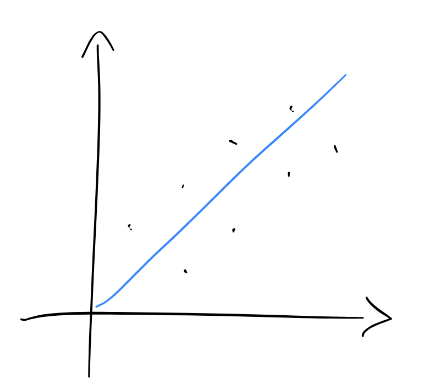
\includegraphics[width=0.9\linewidth]{Pictures/Schermata_20251209_184020.png}
    \captionof*{figure}{\small LS minimization visualization}
\end{minipage}

\vspace{0.5cm}

\noindent
\begin{minipage}{0.65\textwidth}
    Since \colorbox{yellow!20}{we know the symbol we've sent and we know its power}, \colorbox{yellow!20}{we can learn the} \colorbox{yellow!20}{response of the channel accordingly.}
    
    We can model the received signal as
    \begin{align*}
        y[n] = \sqrt{G} \sum_{\ell=0}^{L} H[\ell]x[n-\ell] + v[n].
    \end{align*}
\end{minipage}%
\hfill
\begin{minipage}{0.3\textwidth}
    % Note manoscritte in alto a destra nella pagina originale
    \footnotesize
    \textcolor{purple}{\textbf{Formal writing:}}
    \begin{align*}
        \mathrm{y}[k] &= \sqrt{G} \mathrm{h}[k] \mathrm{p}[k] + \mathrm{v}[k] \\
        &\quad \uparrow \quad \quad \quad \uparrow \\
        &\text{useful} \quad \text{noise}
    \end{align*}
\end{minipage}

\section*{How the \textit{H} matrices represent the delay}

Let's suppose we have 2 transmit and 2 receive antennas and all the signals arrive without any delay at the receiver:

\begin{figure}[h]
    \centering
    % Diagramma MIMO 2x2 flat (frecce nere dirette)
    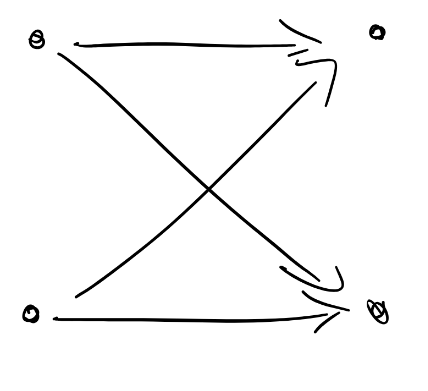
\includegraphics[width=0.4\textwidth]{Pictures/Schermata_20251209_184043.png}
    \caption*{2x2 MIMO with no delay}
\end{figure}

We'll use a matrix such as
\begin{align*}
    \boldsymbol{H} = \begin{bmatrix} h_{00} & h_{01} \\ h_{10} & h_{11} \end{bmatrix}
\end{align*}
to characterize the channel.

Even in this case, there could be other paths, with different delays!

\begin{figure}[h]
    \centering
    % Diagramma MIMO 2x2 con percorsi diretti (0) e riflessi (1, frecce blu)
    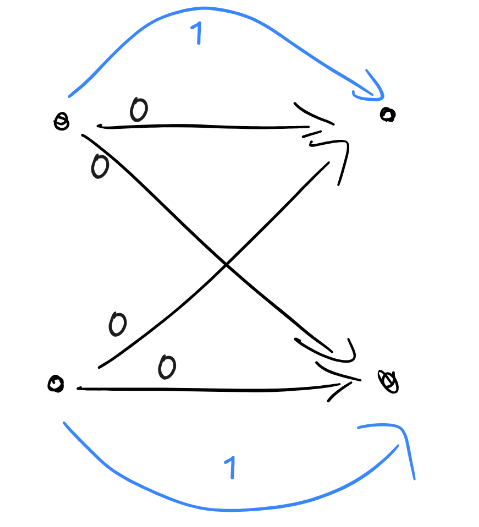
\includegraphics[width=0.4\textwidth]{Pictures/Schermata_20251209_184057.png}
    \caption*{MIMO paths with different delays (blue arrows arrive at time 1)}
\end{figure}

Here the channel won't be flat anymore (the arrows in blue arrive at time 1): the one before will be

\begin{align*}
    \boldsymbol{H}(0) = \begin{bmatrix} h_{00}(0) & h_{01}(0) \\ h_{10}(0) & h_{11}(0) \end{bmatrix}
\end{align*}

and we'd also have

\begin{align*}
    \boldsymbol{H}(1) = \begin{bmatrix} h_{00}(1) & 0 \\ 0 & h_{11}(1) \end{bmatrix}:
\end{align*}

we have some form of reflection which makes the signal arrive later at the receiver.
Of course if we were to have reflections between 0,1 and 1,0, we'd have

\begin{align*}
    \boldsymbol{H}(1) = \begin{bmatrix} h_{00}(1) & h_{01}(1) \\ h_{10}(1) & h_{11}(1) \end{bmatrix}.
\end{align*}

\end{document}